\documentclass[10pt,a4paper]{article}
\usepackage[utf8]{inputenc}
\usepackage[T1]{fontenc}
\usepackage[a4paper]{geometry}
\usepackage{amsmath}
\usepackage{amssymb}
\usepackage{bm}
\usepackage{IEEEtrantools}
\usepackage{multicol}
\usepackage{graphicx}
\usepackage{float}
\usepackage{url}
\usepackage{subcaption}

\author{
  Chakraborty, Upasana \\
  \texttt{uchakrabo@student.ethz.ch}
  \and
  Kapoor, Mohit \\
  \texttt{mkapoor@student.ethz.ch}
  \and
  Karpf, Michael \\
  \texttt{mkarpf@student.ethz.ch}
  \and
  Wernli, Florian \\
  \texttt{fwernli@student.ethz.ch}
}
\title{Multi User MIMO}

\begin{document}
\maketitle
%\begin{multicols}{2}
	
\noindent The sum-rate for the three scenarios can be calculated like below:
	\begin{itemize}
		\item MU-MIMO: $C=\log_2\left(\det\left[\textbf{I}_{M_R}+\textbf{H}\textbf{H}^H\right]\right)$
		\item Orthogonalization: $C=\sum_{i=1}^{M_T}\frac{1}{M_T}\log_2\left(\det\left[\textbf{I}_{M_R}+\textbf{H}_i\textbf{H}_i^H\right]\right)$
		\item Interference \cite{bib:interference}: $C=\sum_{i=1}^{M_T}\left\{\log_2\left(\det\left[\textbf{I}_{M_R}+\textbf{H}\textbf{H}^H\right]\right)-\log_2\left(\det\left[\textbf{I}_{M_R}+\sum_{j=1,j\ne i}^{M_T}\textbf{H}_j\textbf{H}_j^H\right]\right)\right\}$
                \end{itemize}      
                Where $\textbf{H}$ is a $M_R\times M_T$ channel matrix, whereby we assume i.i.d. Rayleigh fading $h_{m,n}\sim\mathcal{CN}(0,1)$ for all entries. The SNR is 0 dB.
	\paragraph{8 receive antennas} lead to the results depicted in figure \ref{fig:res_8}. The highest sum-rate is achieved with successive interference cancelling in a MU-MIMO setting. Not quite as good are the achieved sum-rates when we treat all other senders as interference and the worst results are achieved by using an orthogonalization approach (i.e. TDD). In case of SIC only the data rate of the first sender has to be low enough to cope with the interference from all other senders while the rest of the senders experience less and less interference due to the cancelling at the receiver. This larger influence of interference for 7 out of 8 sender leads to the lower sum-rates. The bad results from the orthogonalization approach are due to the long time the senders are inactive. The more sender we have, the less time each sender gets to use the channel (i.e. the senders are inactive $\frac{7}{8}$ of the time in our case) and since the factor is outside of the $\log_2$ expression the data-rate decreases linearly with an increasing number of senders. 
	
	\paragraph{80 receive antennas} show a similar behaviour (figure \ref{fig:res_80}). The MU-MIMO case still achieves the best results followed by the interference scenario and the orthogonalization scenario in the last place. However, the MU-MIMO and interference scenario are now almost identical while having more than doubled the sum-rate. Due to the law of large numbers, combining the received signals averages out the interference terms leading to a receive signal with almost no interference. The MU-MIMO and interference scenario thus perform both optimally without any significant interference when we increase the number of receive antennas by a large number. The sum-rate in the orthogonalized scenario increases too, but only by a small amount since we didn't have interference in the first place and only profit from an increased array-gain at the receiver. Additionally, in all three cases we see much steeper curves indicating a much lower variance of the instantaneous sum-rates. This is again due to the large number of antennas averaging out the sum-rate.
	
	\begin{figure}
		\begin{subfigure}{0.5\textwidth}

			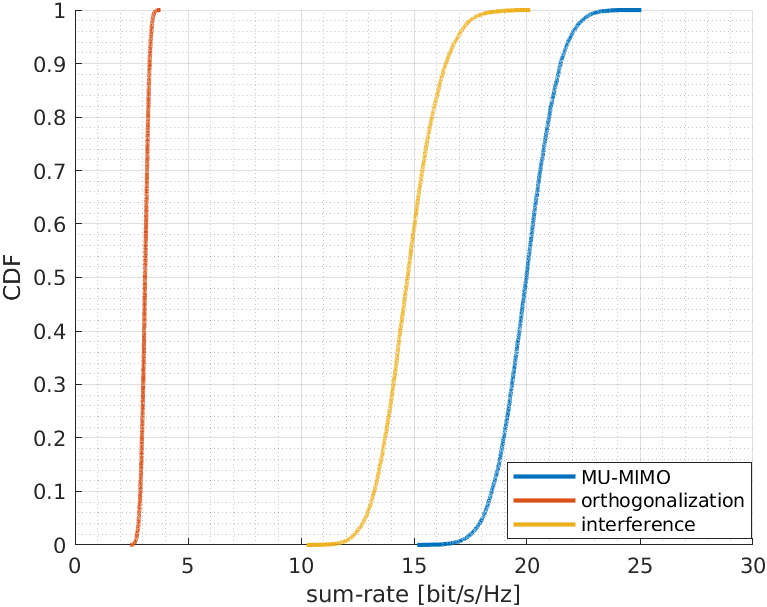
\includegraphics[width=\textwidth]{result.png}

			\subcaption{8 receive antennas}

			\label{fig:res_8}

		\end{subfigure}
		\begin{subfigure}{0.5\textwidth}

			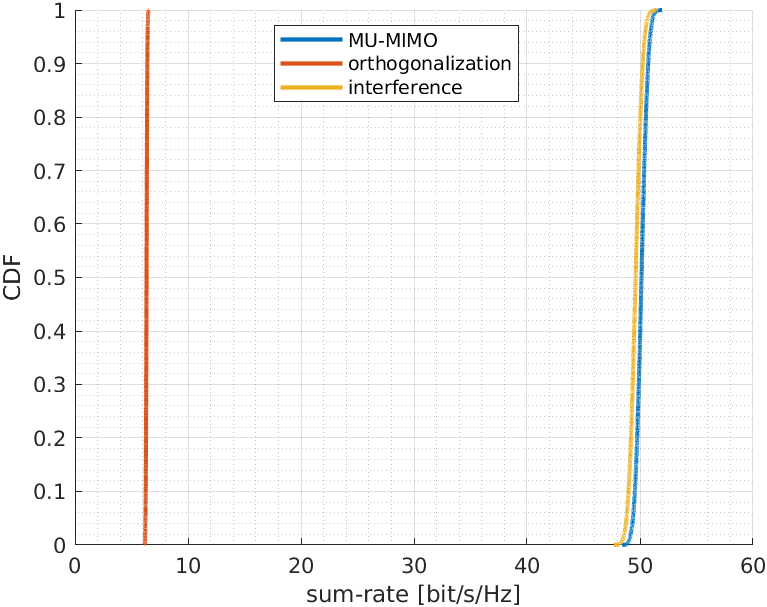
\includegraphics[width=\textwidth]{result_80.png}

			\subcaption{80 receive antennas}

			\label{fig:res_80}

		\end{subfigure}

		\caption{achievable sum-rate}

		\label{fig:res}

	\end{figure}

  \bibliographystyle{ieeetr}
  \bibliography{bib}
%\end{multicols}
\end{document}
